% chktex-file 13

\documentclass{article}
\usepackage{amsmath}
\usepackage{hyperref}
\usepackage{xcolor}
\usepackage{ulem}
\usepackage{graphicx}
\usepackage[margin=0.75in]{geometry}

\graphicspath{ {./images/} }

\definecolor{darkblue}{rgb}{0, 0, 20}

\hypersetup{
    colorlinks=true,
    urlcolor=darkblue,
    linkcolor=blue,
    filecolor=magenta,
    citecolor=blue,
}

\title{HOISDF:\@ Constraining 3D Hand-Object Pose Estimation with Global Signed Distance Fields}
\author{Haozhe Qi, Chen Zhao, Mathieu Salzmann, Alexander Mathis}
\date{}
\setlength{\parindent}{0pt}

\begin{document}

\maketitle

\begin{center}\textbf{Accepted for CVPR 2024 (\href{https://arxiv.org/pdf/2402.17062}{Paper}) (\href{https://github.com/amathislab/HOISDF}{GitHub})}\end{center}

The HOISDF model estimates signed distance fields for both the hand and object to build the shape of each with sampled points. The sample points on the surface are then used to predict hand joints and shape, as well as object rotation and translation.

\begin{center}
    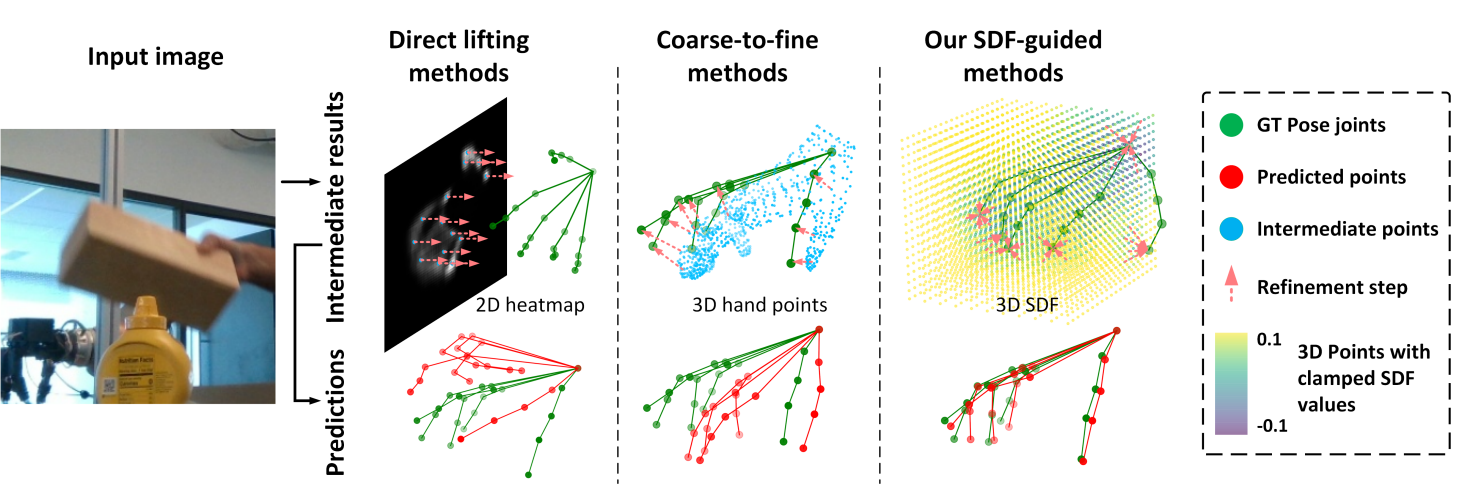
\includegraphics[scale=0.4]{hoisdf-1.png}
\end{center}

\section*{Motivation}
This model encodes the hand shape as a continuous function instead of a surface mesh with predefined vertices and edges. Also, since the pose keypoints are determined from the signed distance field, you have more freedom around the keypoint prediction by modifying the signed distance field decoder, such as joint or collision constraints.

\begin{center}
    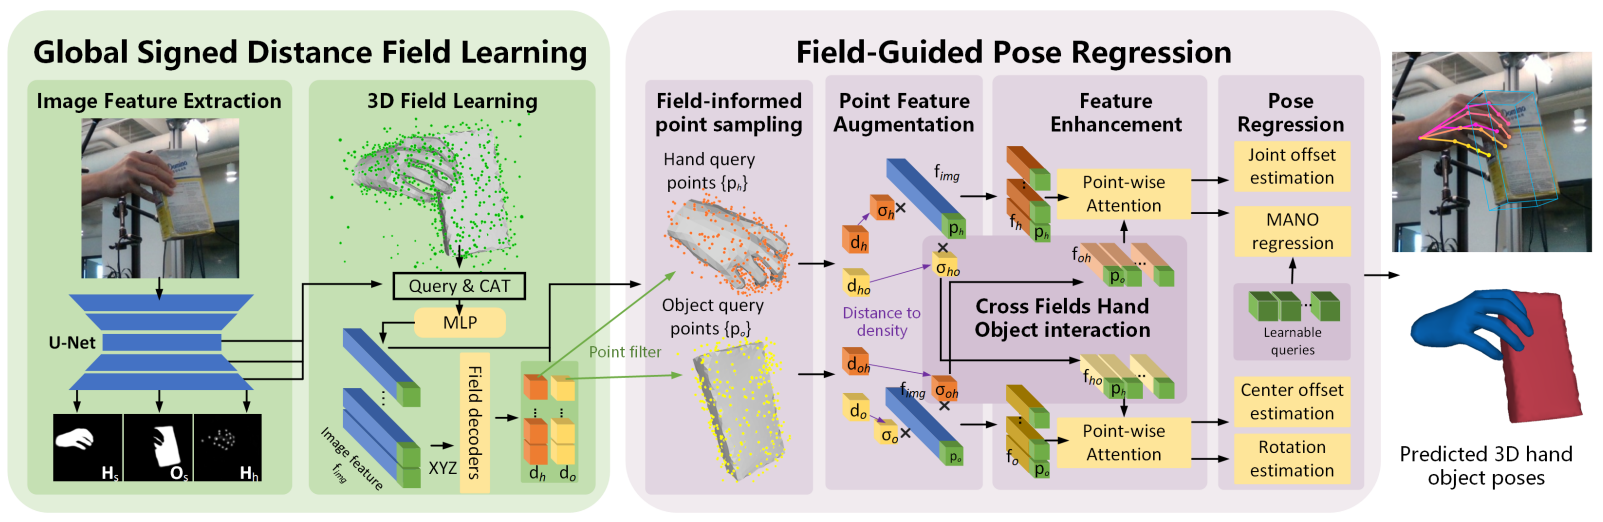
\includegraphics[scale=0.4]{hoisdf-2.png}
\end{center}

\section*{Method}

\subsubsection*{Global Signed Distance Field Learning}
\begin{enumerate}
    \item \textbf{Image Feature Extraction}
    
    A U-Net architecture extracts hand and object segmentation masks and 2D keypoint predictions from the image.

    \item \textbf{3D Signed Distance Field Learning}
    
    The decoder part of the U-Net is then used to convert a 3D point into an image feature vector. Fourier positional encoding is also incorporated to expand the 3D point to a larger space. The 3D point, image features, and positional encodings are passed through a fully connected neural network to predict the signed distance to the hand or object surface with positive values for outside of the hand and negative for inside.
\end{enumerate}

\subsubsection*{Field-Guided Pose Regression}
\begin{enumerate}
    \item \textbf{Field-informed Point Sampling}
    
    The 3D space is split into uniform bins, each with a query point, and then the points are filtered in the 2D space using the hand and object bounding boxes. The points are sorted using their distances to the surface and the first set of points are kept.
    
    \item \textbf{Field-based Point Feature Augmentation}
    
    For each query point, its volume density is calculated where a higher density is closer to the surface, giving more importance to those points. This is concatenated with the features from before to form the final query point feature vector.

    \item \textbf{Cross Fields Hand-Object Interaction}
    
    The query points are passed through the other signed distance field so hand query points are passed through object signed distance field and vice versa. We then repeat what we did before but with these distances instead.

    \item \textbf{Feature Enhancement with Point-wise Attention}
    
    The final feature and cross-field feature vectors are passed through six multi head self-attention layers to compute the enhanced point features.

    \item \textbf{Point-wise Pose Regression}
    
    Cross attention layers are used with 17 learned hand pose queries to compute the 3D joint angles and the 10D mano shape parameters. For each joint, distance vectors are created from each nearby query point to the joint to fine-tune that joint’s 3D position. Since the object is more rigid, the rotation and translation vectors can be directly regressed from the enhanced object features.
\end{enumerate}

\begin{center}
    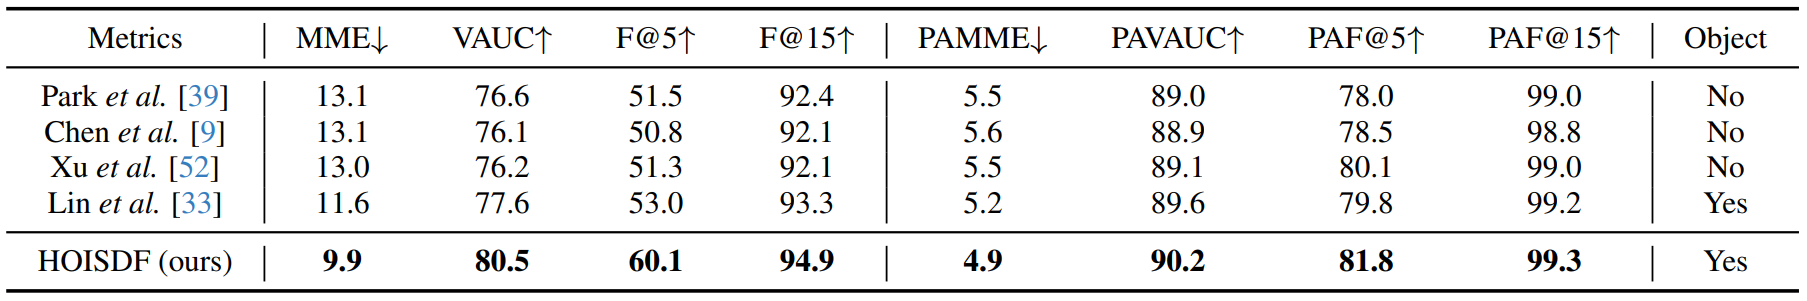
\includegraphics[scale=0.3]{hoisdf-3.png}
\end{center}

\section*{Limitations}

\begin{enumerate}
    \item The paper explicitly states that the hand and object meshes might intersect with each other in severely occluded scenarios. A possible solution is to include a weighted loss value for mesh intersections in the SDF decoder with SDF learning.
    \[L_\text{overlap}=\frac{1}{N}\sum_{p\in P} \text{ReLU}(-\text{SDF}_\text{hand}(p))\cdot \text{ReLU}(-\text{SDF}_\text{object}(p))\]
    \item The two datasets this model was trained on only include objects that are bigger than the hand, which are much less occluded than smaller objects.
\end{enumerate}

\subsubsection*{Enhancements}
\begin{enumerate}
    \item Train a separate temporal transformer encoder module that will receive the keypoint predictions for the video once all of the frames have been calculated and then shifts the keypoints to ensure smooth and consistent transitions.
    \begin{itemize}
        \item Leverages the Multi-Head Self Attention to capture global relationships
        \item Allows the frames to be still processed in parallel by not making each frame dependent on previous frames
    \end{itemize}
    \item Pass the previous keypoints along with the query point to the current SDF decoder.
\end{enumerate}

\end{document}